%This is a template file for use of iopjournal.cls

\documentclass{iopjournal}
\bibliographystyle{IEEEtran}
\usepackage{float}
\usepackage{amsmath}
\usepackage{tikz}
\usepackage{fix-cm} % Allow scalable Computer Modern fonts to avoid font substitution warnings

% Options
%  [anonymous]  Provides output without author names, affiliations or acknowledgments to facilitate double-anonymous peer-review
%
% The following packages are required by iopjournal.cls and do not need to be declared again:
%  graphicx
%  fancyhdr
%  xcolor
%  hyperref
%

\begin{document}

\articletype{Tarea 5} %	 e.g. Paper, Letter, Topical Review...

\title{Descenso de Gradiente de n-Dimensiones}

\author{Daniel González$^1$\orcid{0000-0000-0000-0000}}

\affil{$^1$Facultad de Ingeniería, Universidad Autónoma de Querétaro, Querétaro, México \\ 08/09/2025}

\email{dgonzalez16@alumnos.uaq.mx}

\keywords{descenso gradiente, plano, mínimo, espacio, épocas, n-dimensiones}

\begin{abstract}
El descenso de gradiente es un método iterativo de optimización que utiliza la gradiente para aproximarse al mínimo de una función de costo. En el caso de $n$ características, la gradiente se expresa como un vector de derivadas parciales, donde cada componente representa la dirección de mayor pendiente respecto a una variable. Al avanzar en dirección contraria de ese vector, el algoritmo actualiza los parámetros paso a paso según la regla

\[
\theta_j := \theta_j - \alpha \frac{\partial J(\boldsymbol{\theta})}{\partial \theta_j}, \quad j=1,2,\dots,n,
\]

donde $\alpha$ es la tasa de aprendizaje. De esta manera, se logra descender progresivamente sobre la superficie multidimensional de la función hasta aproximarse a un mínimo local o global.
\end{abstract}

\section{Introducción}

En el aprendizaje automático supervisado, el objetivo es encontrar una función que modele la relación entre un conjunto de características de entrada y una variable de salida. Para ilustrar el proceso, a menudo se comienza con el caso más simple, en el cual el modelo depende de una sola característica. Sin embargo, los problemas reales requieren generalizar a múltiples características, lo que hace necesaria una notación más compacta y eficiente.

Con este propósito, los parámetros del modelo se agrupan en un vector columna
\[
\boldsymbol{\theta} = 
\begin{bmatrix}
\theta_0 \\
\theta_1 \\
\vdots \\
\theta_n
\end{bmatrix},
\]
mientras que las características de los $m$ ejemplos de entrenamiento se organizan en una matriz
\[
X = 
\begin{bmatrix}
x_1^0 & x_1^1 & \cdots & x_1^n \\
x_2^0 & x_2^1 & \cdots & x_2^n \\
\vdots & \vdots & \ddots & \vdots \\
x_m^0 & x_m^1 & \cdots & x_m^n
\end{bmatrix},
\]
donde $x_i^0 = 1$ para todo $i = 1, \dots, m$, lo que permite incorporar el término de sesgo en el modelo.

Bajo esta formulación, la hipótesis se expresa como
\[
h_\theta = X \cdot \boldsymbol{\theta},
\]
que produce un vector de dimensión $m \times 1$ con las predicciones correspondientes a cada ejemplo de entrenamiento.  

Para evaluar la calidad de dichas predicciones se emplea la función de costo basada en el error cuadrático medio (MSE), definida como
\[
J(\theta) = \frac{1}{2m} \sum_{i=1}^{m} \big(h_\theta(x_i) - y_i\big)^2,
\]
la cual, en notación vectorial, puede escribirse como
\[
J(\theta) = \frac{1}{2m} (X \cdot \boldsymbol{\theta} - Y)^T (X \cdot \boldsymbol{\theta} - Y),
\]
donde
\[
Y = 
\begin{bmatrix}
y_1 \\
y_2 \\
\vdots \\
y_m
\end{bmatrix}.
\]

El siguiente paso consiste en optimizar esta función de costo para encontrar los parámetros que mejor se ajustan a los datos. Para ello se utiliza el algoritmo de gradiente descendente, que actualiza los parámetros de manera iterativa siguiendo la regla
\[
\theta_j := \theta_j - \alpha \frac{\partial}{\partial \theta_j} J(\theta), \quad j = 0, 1, \dots, n,
\]
donde $\alpha$ representa la tasa de aprendizaje. El proceso se repite hasta alcanzar la convergencia o completar un número predeterminado de iteraciones, permitiendo aproximarse al mínimo de la función de costo y, por tanto, al modelo más adecuado.


\section{Desarrollo}
\begin{figure}[H]
 \centering
        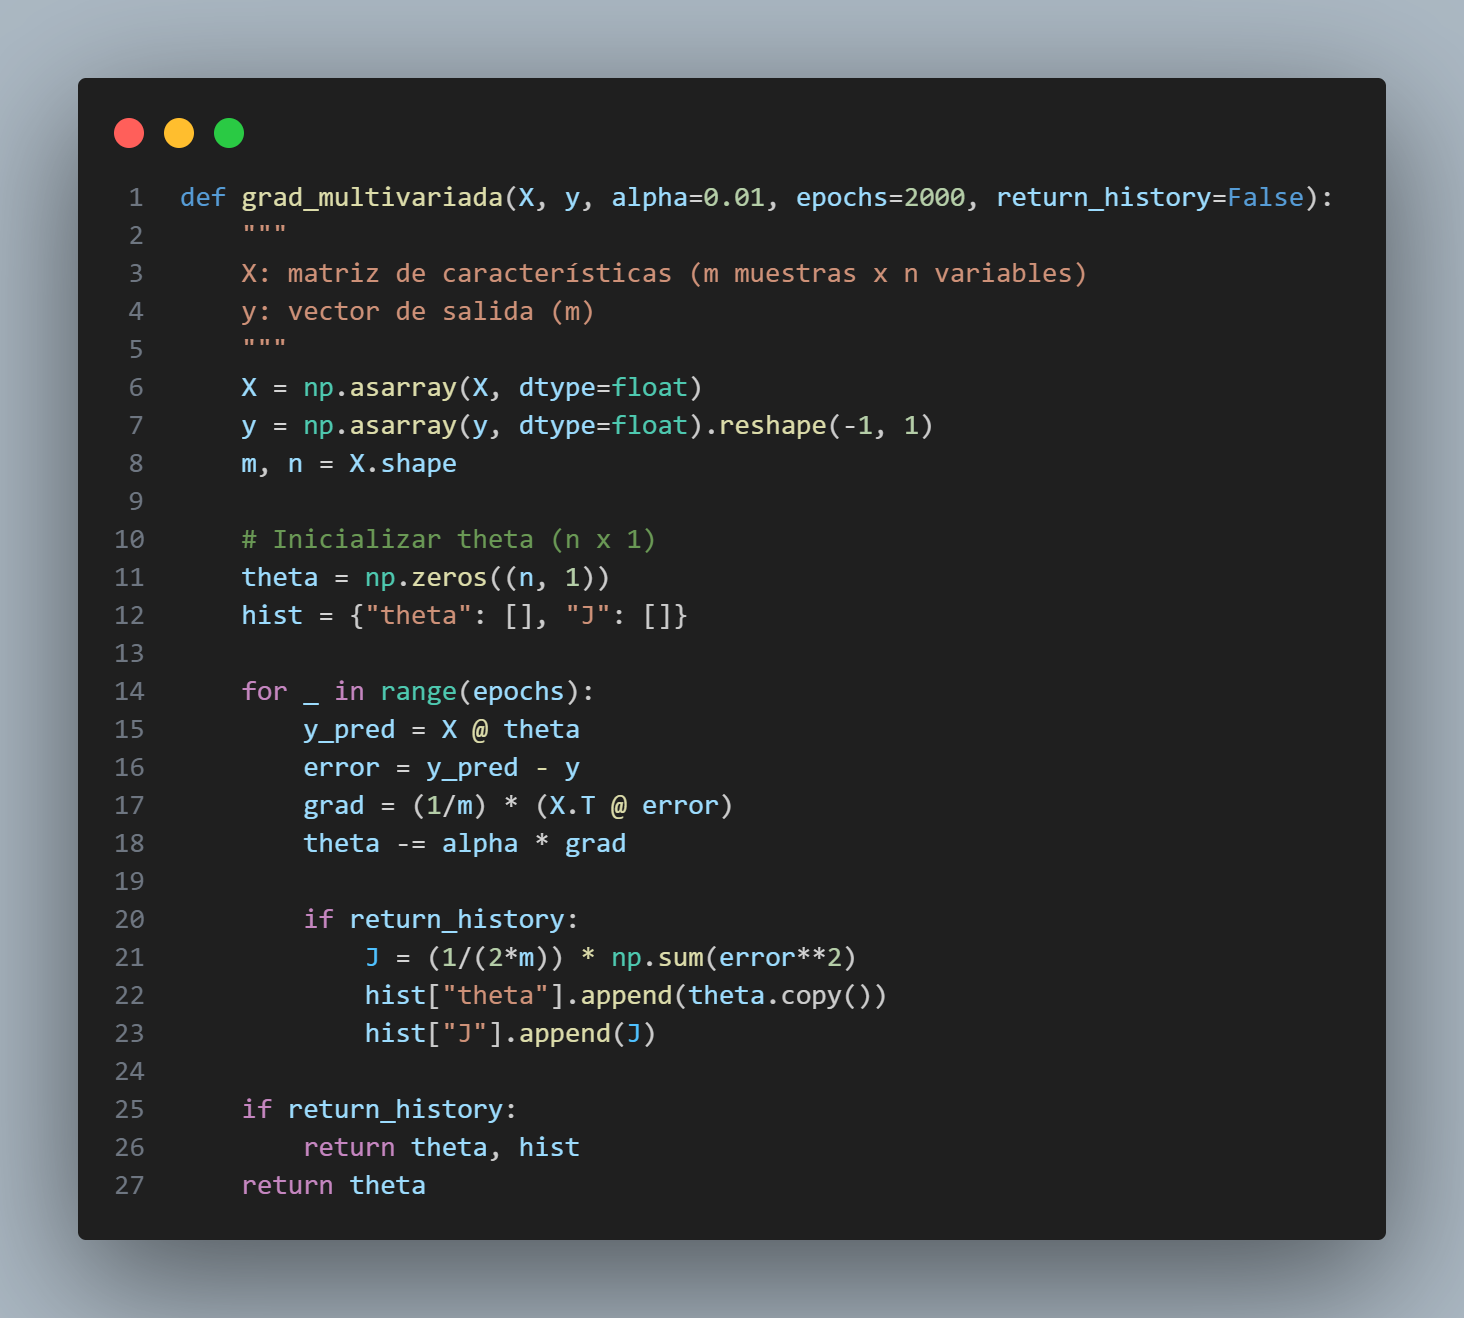
\includegraphics[width=0.5\textwidth]{rsc/funcion_n.png}
 \caption{Funcion para N dimensiones}
\label{fig1}
\end{figure}

A partir de la función propuesta en la figura \ref{fig1}, tomaremos nuestra DB propuesta en problemas anteriores (Advertising.csv) y usaremos como características las 3 columnas de ventas, es decir, TV, Radio y Newspaper.
Recordemos que se crea nuestra matriz de características $X + (Columna de 1s)$ y nuestro vector de etiquetas $Y$ el cual seran nuestras ventas(``Sales'').

Agregaremos tambien la opcion de guardar el hostorico para poder graficar la evolucion de los parametros y la funcion de costo. Ademas de nuestro 
Error cuadratico medio (MSE) que nos ayudara a que es la mejor solucion.

Con esto obtenemos lo siguiente:

\begin{figure}[H]
 \centering
        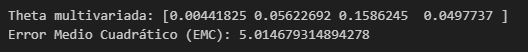
\includegraphics[width=0.5\textwidth]{rsc/Resultados.png}
 \caption{Resultados del modelo}
\label{fig2}
\end{figure}

Dado que al ser un hyperplano en 4 dimensiones no podemos graficar la funcion de costo, pero si podemos ver la evolucion de los parametros y 
el error cuadratico medio (MSE) en la figura \ref{fig3}.

\begin{figure}[H]
 \centering
        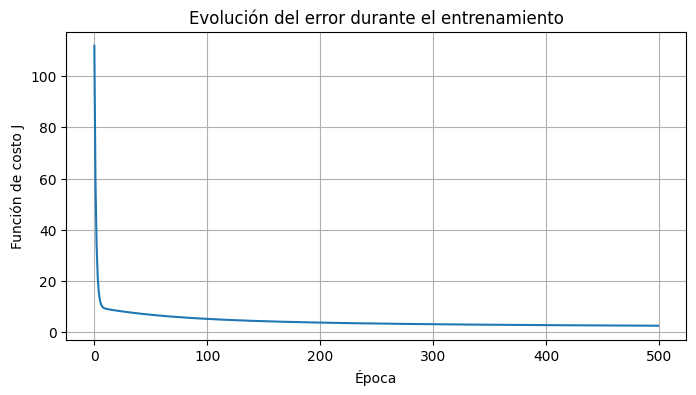
\includegraphics[width=0.5\textwidth]{rsc/Grafica_Error.png}
 \caption{Evolución del MSE}
\label{fig3}
\end{figure}

Como ejercicio complementario a nuestro ejercicio de n-Dimensiones, calculamos el descenso de gradiente para 2 variables, es decir,
una funcion en 3 dimensiones la cual nos muestra un plano en el espacio tridimensional.
\begin{figure}[H]
 \centering
        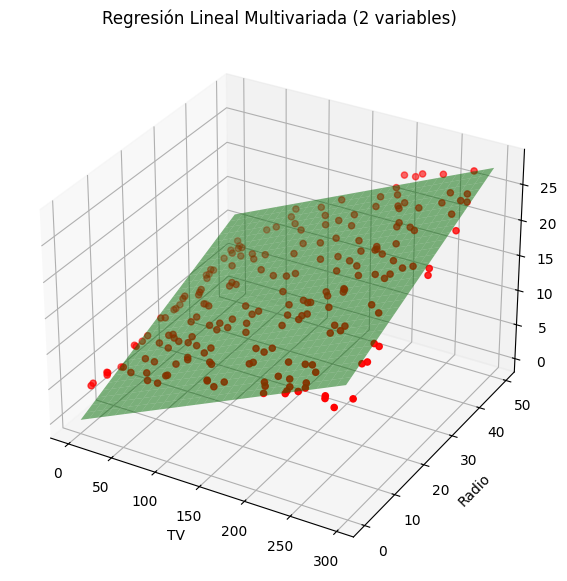
\includegraphics[width=0.5\textwidth]{rsc/Espacio_3D.png}
 \caption{Regresion Lineal en 3D de 2 variables}
\label{fig4}
\end{figure}

\section{Conclusión}

La formulación vectorizada del modelo lineal permite generalizar de manera eficiente el uso de múltiples características en problemas de aprendizaje automático.
Al expresar la hipótesis y la función de costo en notación matricial, se facilita la implementación computacional y se optimiza el cálculo en grandes volúmenes de datos.
Con esto determinamos que el algoritmo de gradiente descendente es una herramienta fundamental para ajustar los parámetros de nuestro modelo, 
garantizando un entrenamiento más eficiente.

%\begin{thebibliography}{00}
%\bibliography{references}
%\end{thebibliography}


\end{document}


